\section{Aperture Photometry Calibration}% {\color{green} Jean-Fran\c cois}}

The total flux density of a source can be measured in the NIKA2 map
over a large circular aperture to recover the source power incident on the telescope through its main
beam as well as its side lobes. It is computed as :

\begin{equation}
S(\nu) = \sum_{m} \sum_{n}  I_{m,n} ({\rm Jy/beam}) \times {dx^2 \over {\Omega_{tot}(\nu)}}
\label{eq:ApPh_7_7}
\end{equation}

\noindent  $I_{m,n}$ is the brightness map in Jy/beam measured in the
map pixel $(m,n)$; $dx$ is the pixel size \samu{as defined by the chosen map resolution;}
$\Omega_{tot}$ is the solid angle of the {\it total} beam; pixel
indices ($m,n$) are such that the radial distance $dx \times
\sqrt{(m-m_c)^2 + (n-n_c)^2}$ from the map center $(m_c,n_c)$
is within the aperture radius. 

Since flux density uncertainty grows with aperture radius, we have
tested various aperture size from $60''$ to $250''$ and found that
$150''$ is a good compromise between
uncertainty and full saturation of the flux density (see Figure
\ref{fig:Uranus_s308}).
%We note however that the power unaccounted for beyond an aperture radius
%of $250''$ is about 30\% at 260 GHz in using parameters in Tables 1
%and 2 of \cite{Kramer2013}.
We note however that \new{the relative power stemming from the second and
third error beams and from the forward and rearward spillowers, hence
which are unaccounted for beyond an aperture radius
of $150''$, is of $24\%$ at $145\, \rm{GHz}$ and of 38\% at $230\,
\rm{GHz}$ in using the beam pattern parameters fitted using EMIR measurements of the
limb of the Moon~\cite{Kramer2013}.}

%(amplitudes of the three error beams at 280GHz and 210GHz,
%$\eta_{fss}$ and 1-Feff and Carsten's email).

The brightness map $I_{m,n}$ in Eq.~\ref{eq:ApPh_7_7} is in unit of
Jy/beam, where {\it beam} stands for the {\it total} beam.
Hence, prior to summing all \samu{map pixels} within the aperture, $I_{m,n}$
must be converted from  Jy/beam to Jy/pixel. This
conversion is done with the factor $dx^2 \over {\Omega_{tot}}$
which is, effectively, the pixel area $dx^2$ in unit of fractional
beam. 

The solid angle of the total beam $\Omega_{tot}$ \new{has been assumed
  stable against the observing conditions} and taken as the mean value computed from the series of 75
\bm\ scans of Uranus and Neptune, as described in Sect.~\ref{se:beam_efficiency}.
%observations of Uranus and Neptune of runs 9, 12, and 14 at
%elevations between $45^{\circ}$ and $65^{\circ}$.
%It is : 
%\begin{equation}
% \Omega_{tot} (r_{max}, \nu) = \int_0^{r_{max}} B(r, \nu) 2 \pi r dr
%\label{eq:Otrue}
%\end{equation}

%\noindent where $B(r, \nu)$ is the full beam profile as defined in
%Sect.~\ref{se:fullbeam_prof} and has been obtained in azimuthally averaging brigthness over narrow annuli
%$dr$ in width, and normalised so that B(0)=1 (see e.g. \cite{remithese}).
%We have used $r_{max}=180''$ which is the maximum extent allowed for
%uniform rms in the maps acquired during observations of N2R9, N2R12
%and N2R14.
Results are given in Tab.~\ref{tab:solid} and are also
copied below in Tab.~\ref{tab:solid_copy} for the reader's convenience. 

The excess of the total beam relative to the Gaussian main beam is the ratio
$\Omega_{tot} / 2 \pi (\sigma_{Gauss})^2$, with $\sigma_{Gauss}$
derived from the $FWHM$ of the main beam determined using the
sidelobe-masked 1D method in Sect.~\ref{se:MB}.

%Observations of Uranus and Neptune during runs 9, 12 and 14 have been used to estimate $\Omega_{tot}$ and results
%are in Table \ref{tab:solid}. The mean values in this Table have been
%adopted for aperture photometry of secondary calibrators presented
%below.

\begin{figure}[ht!]
  \begin{center}
    %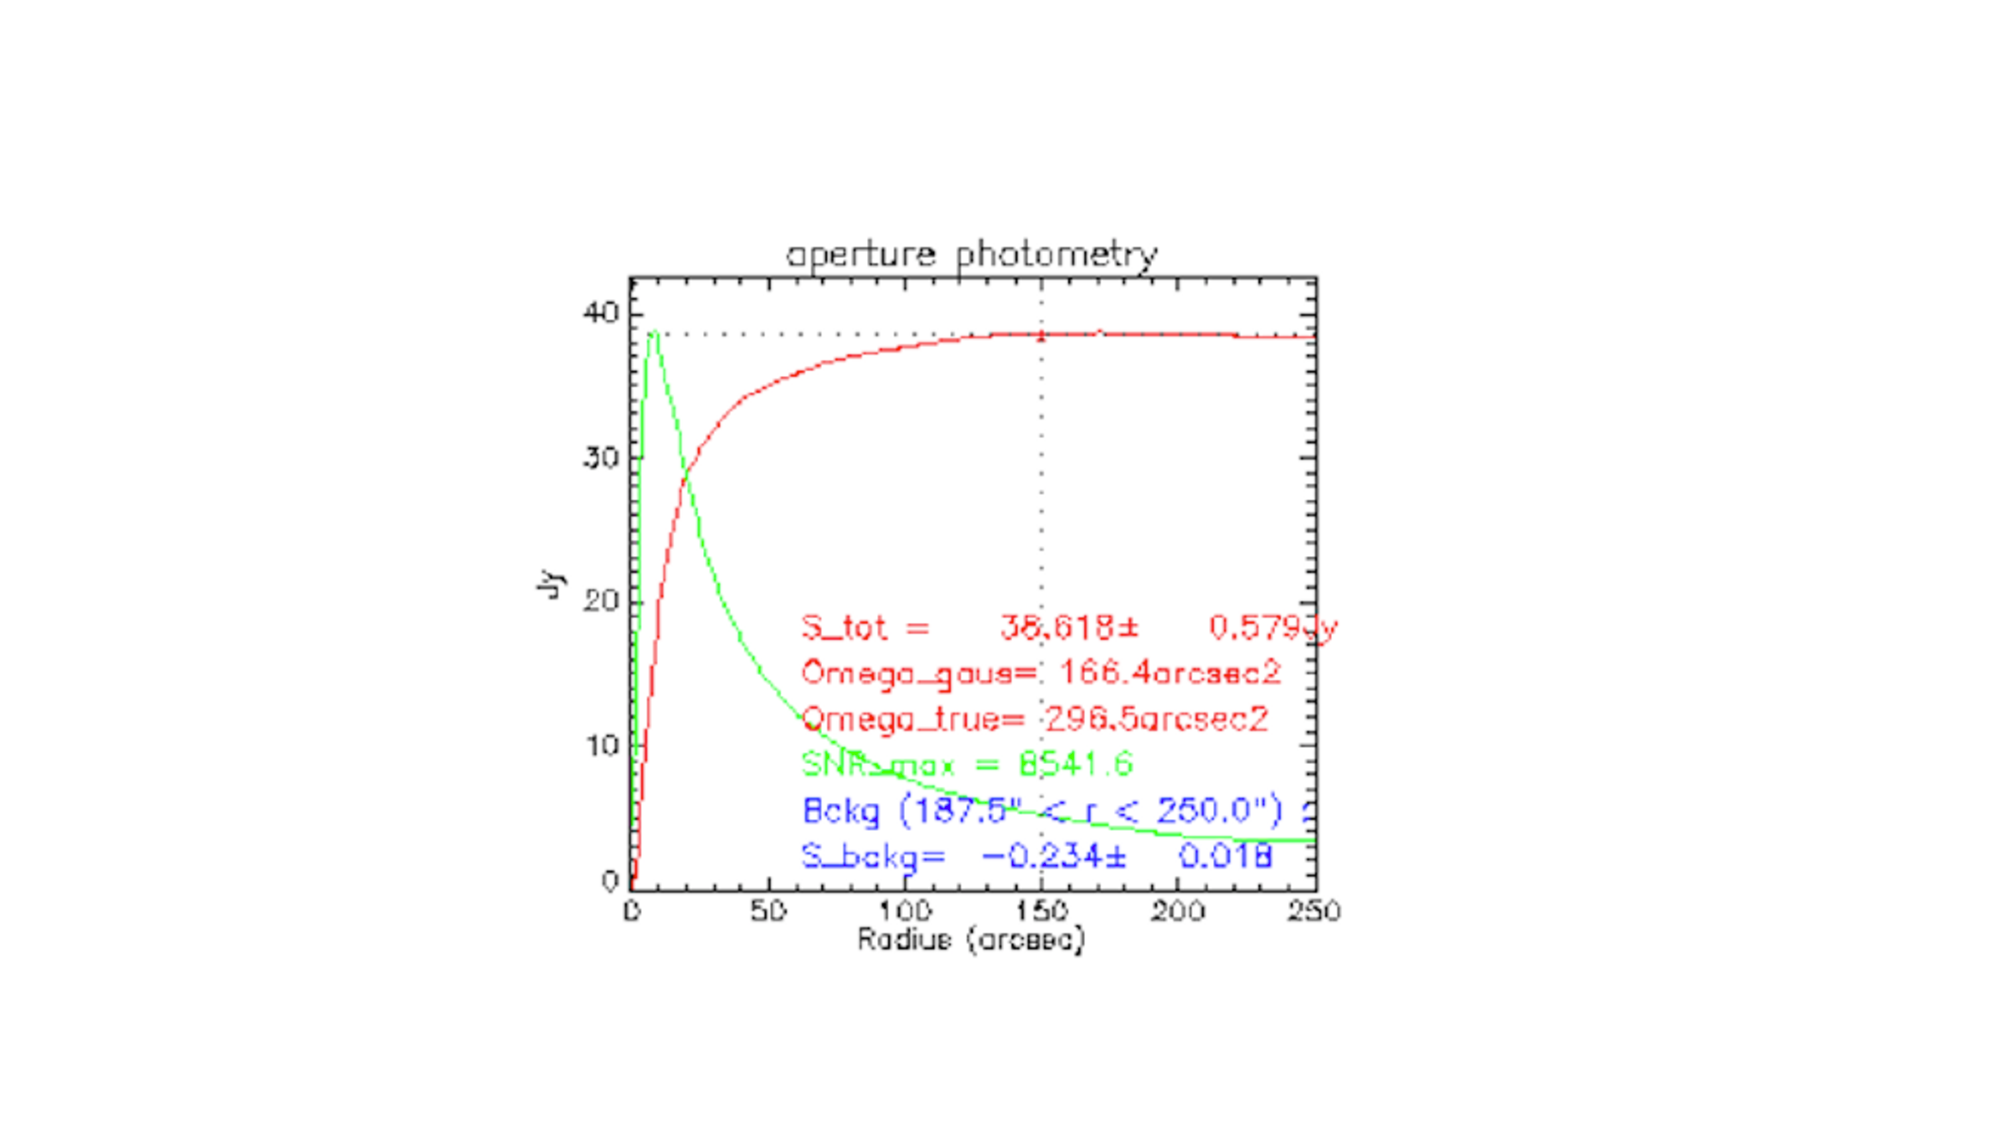
\includegraphics[clip=true,width=0.3\textwidth, trim={8cm, 3cm, 8cm, 4cm}]{Figures/Aperture_photo/Uranus_s308_A1.pdf}
    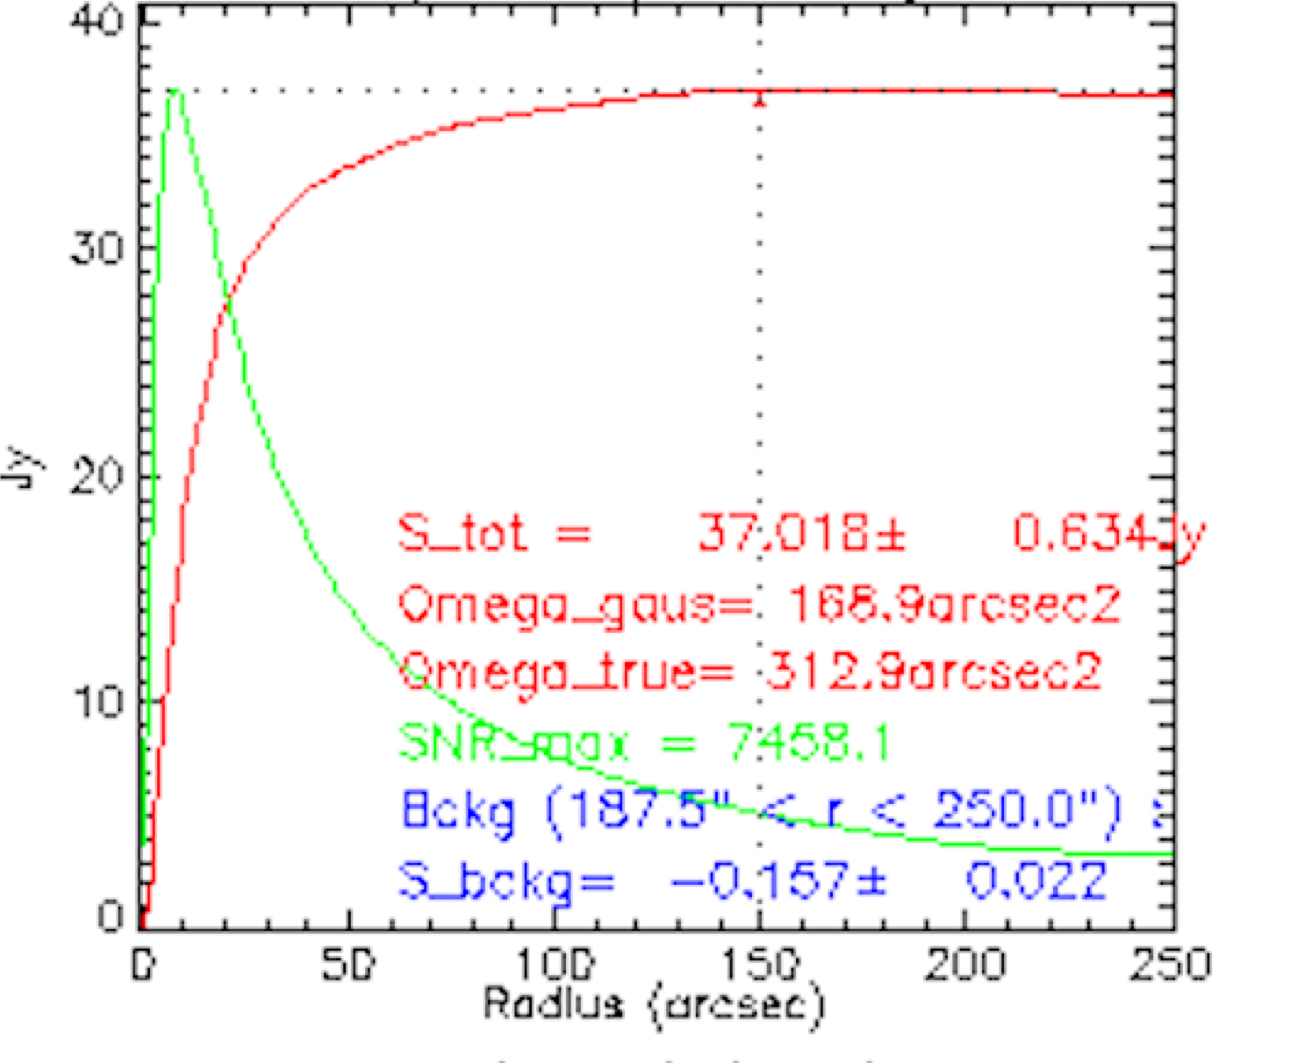
\includegraphics[clip=true,width=0.3\textwidth]{Figures/Aperture_photo/ura_a1.png}
    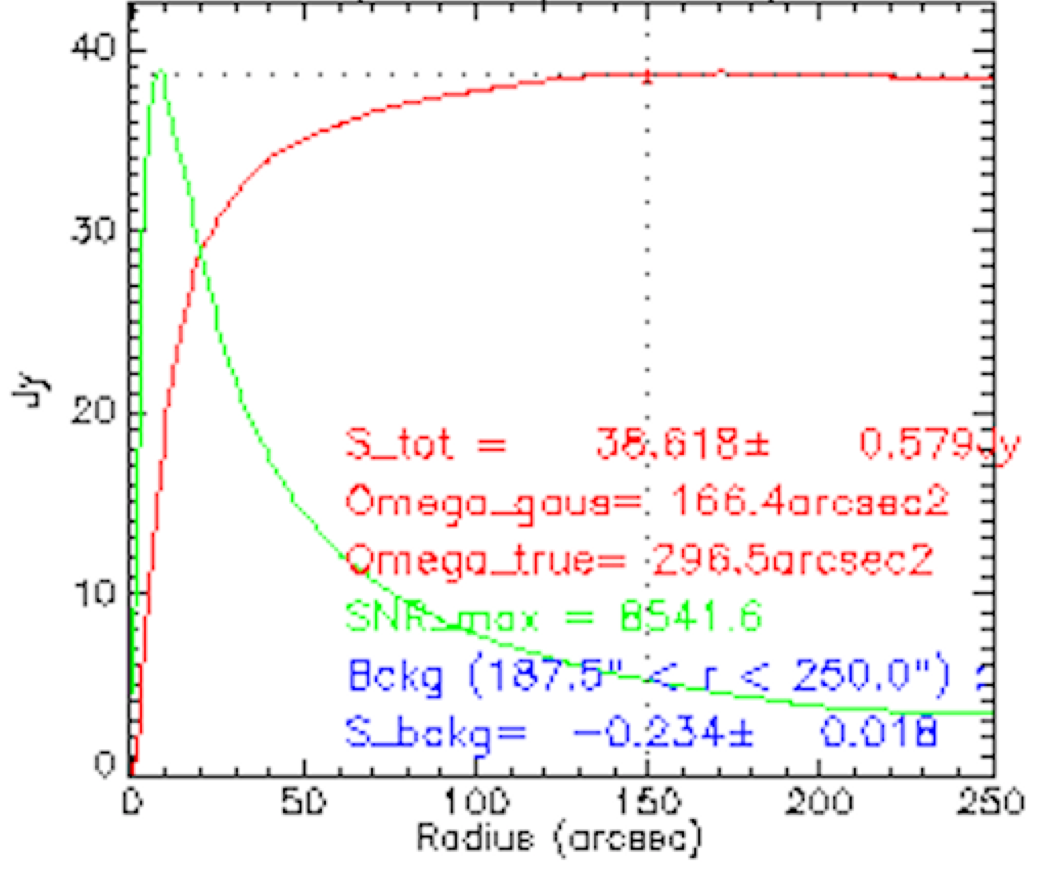
\includegraphics[clip=true,width=0.293\textwidth]{Figures/Aperture_photo/ura_a3.png}
    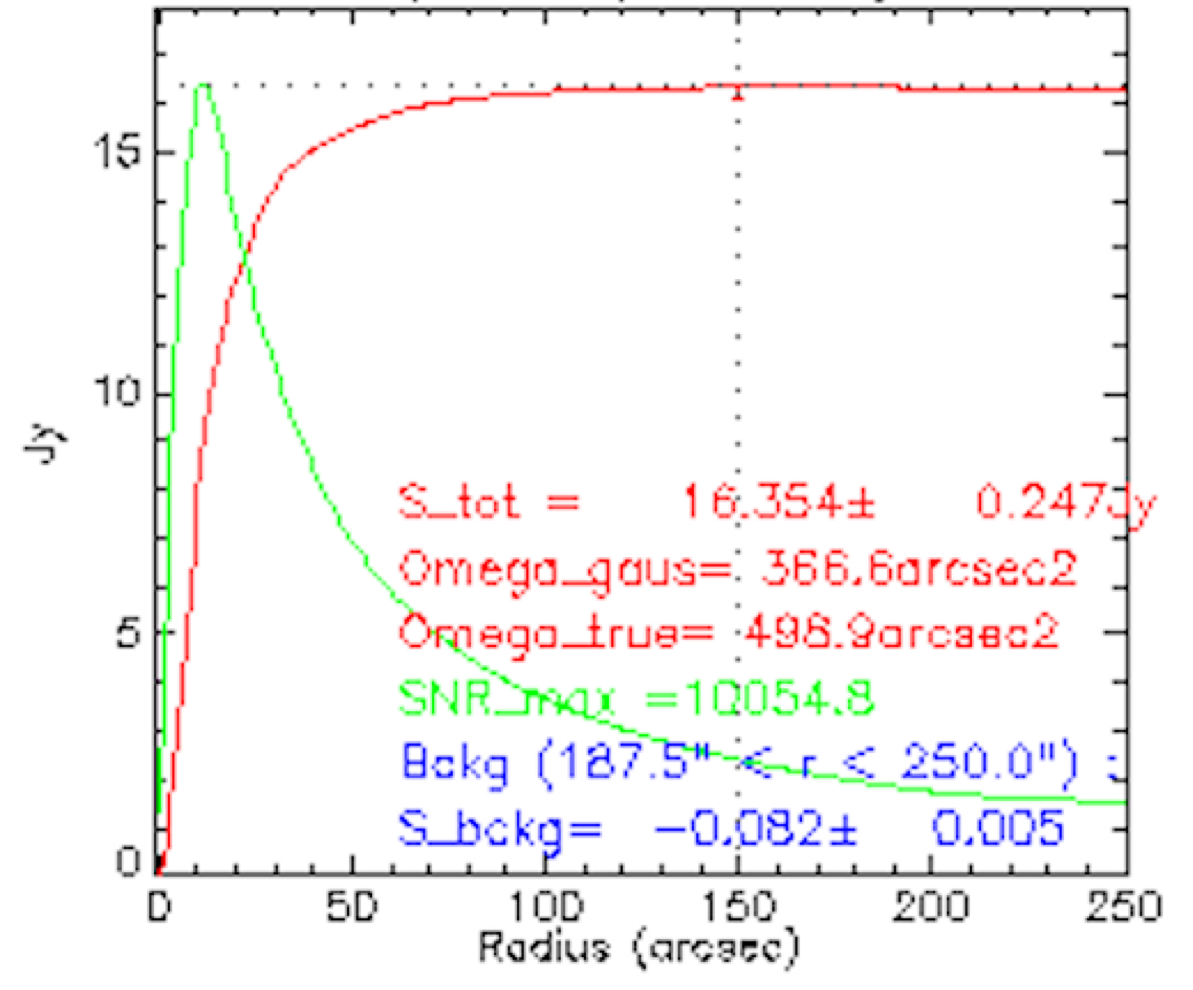
\includegraphics[clip=true,width=0.3\textwidth]{Figures/Aperture_photo/ura_a2.png}
    \caption[Aperture photometry of Uranus]{Example of aperture photometry using a scan of Uranus (20170227s308) acquired during the N2R9 campaign for Array 1, 3 and 2. Integrated flux density is the red curve that saturates at an aperture radius of $ \sim 150''$. Uncertainty over this aperture is $\sim$ 2\% of the total flux density. \todo{Alessia's
    comment: could you improve the resolution of the plot ?}}
    \label{fig:Uranus_s308}
  \end{center}
\end{figure}

\begin{table*}[!h]
\caption{Solid angle of total beam based on Uranus and Neptune observations}
\label{tab:solid_copy}
\centering
\begin{tabular}{l| c | c c c | c c c}
\hline\hline
\noalign{\smallskip}
run  & Nber of scans & \multicolumn{3}{c}{$\Omega_{tot}$ (arcsec$^{2}$)} & \multicolumn{3}{c}{$\Omega_{tot}/\Omega_{gauss}$} \\
\hline
     &               &  A1    &    A2   &  A3  & A1  &  A2  & A3   \\
            \hline
r9    & 27  &  265$\pm$ 23    &  466$\pm$ 17 & 252 $\pm$ 23 &  1.80 $\pm$ 0.12    &  1.35 $\pm$ 0.05   &   1.74 $\pm$ 0.13   \\
r12   & 20  &  229$\pm$ 11    &  437$\pm$  9 & 221 $\pm$ 10 &  1.71 $\pm$ 0.06   &  1.30 $\pm$ 0.02   &   1.68 $\pm$ 0.06   \\
r14   & 28  &  251$\pm$ 16    &  457$\pm$ 15 & 245 $\pm$ 18 &  1.73 $\pm$ 0.08   &  1.32 $\pm$ 0.03   &   1.72 $\pm$ 0.08   \\
mean  &     &  248            &  453         &  239         &  1.74              &   1.32             &   1.71              \\
       \noalign{\smallskip}
            \hline
\end{tabular}
\end{table*}

%If the main beam efficiency is defined as the ratio between the power in the gaussian main beam fitted and
%all the power out to $r_{max}=180''$, it is easy to show that this efficiency is the $ 1 / (\Omega_{tot}/\Omega_{gauss}$).
%These efficiences for the three arrays are provided in Table \ref{tab:MB} as well as the level of the error beam (side lobes)
%relative to the main beam peak in dB (we recall that -12dB as found is 6\%).

%\begin{table*}[!h]
%\caption{Main beam efficiency (\%) and level of error beam (dB)}
%\label{tab:MB}
%\centering
%\begin{tabular}{l| c | c c c | c c c}
%\hline\hline
%\noalign{\smallskip}
%run  & Nber of scans & \multicolumn{3}{c}{Main beam efficiency } & \multicolumn{3}{c}{Error beam level (dB)} \\
%\hline
%     &               &  A1    &    A2   &  A3  & A1  &  A2  & A3   \\
%            \hline
%r9    & 27  &  54.1$\pm$ 3.2\%    &  74.7$\pm$ 2.9\% & 55.9 $\pm$ 3.7\%   &  -11.5 $\pm$ 0.8    &  -14.9 $\pm$ 0.6   &  -12.0 $\pm$ 0.6  \
% \\
%r12   & 20  &  55.7$\pm$ 2.0\%    &  77.4$\pm$ 1.0\% & 57.1 $\pm$ 2.0\%   &  -13.4 $\pm$ 0.3    &  -16.1 $\pm$ 0.3   &  -13.8 $\pm$ 0.3  \
% \\
%r14   & 28  &  55.0$\pm$ 2.7\%    &  76.0$\pm$ 1.8\% & 56.1 $\pm$ 2.6\%   &  -12.5 $\pm$ 0.6    &  -15.3 $\pm$ 0.6   &  -12.7 $\pm$ 0.8  \
% \\
%            \noalign{\smallskip}
%            \hline
%\end{tabular}
%\end{table*}


%  LP
%  --> petite introduction temporaire : peut etre modifiee/effacee
%To be discussed in this section: the aperture photometry method, the conversion factor between Gaussian Beam photometry and aperture photometry and as example, some stability tests on Planets using aperture photometry

%The aperture photometry method that was used to derive the first calibration results as reported in~\cite{Adam18} is detailed in Sect.~\ref{ap:cal_JFL}. 


%  JFL
%  --> extracted from results_Ap.tex

Finally, in Table~\ref{tab:ratio}, we provide the ratio between the
flux densities derived by aperture photometry
and derived using the fixed-width Gaussian photometry, as defined in
Sect.~\ref{se:flux_density_equation}.
%by a simple Gaussian fit to the source (Uranus or Neptune) with the fixed fwhms $12.5''$ and $18.0''$
%at 1mm and 2mm.
These ratios are larger than unity and indicate that aperture
photometry recovers more flux density than a Gaussian fit as
expected.

%A full analysis of these ratios would require to take into
%account the fact that KIDs (kidpars) have actually been calibrated by
%fitting a fixed gaussian to Uranusor Neptune. Hence, there is a slight
%inconsistency in applying aperture photometry in these conditions.


%\begin{figure}[ht!]
% \begin{center}
%  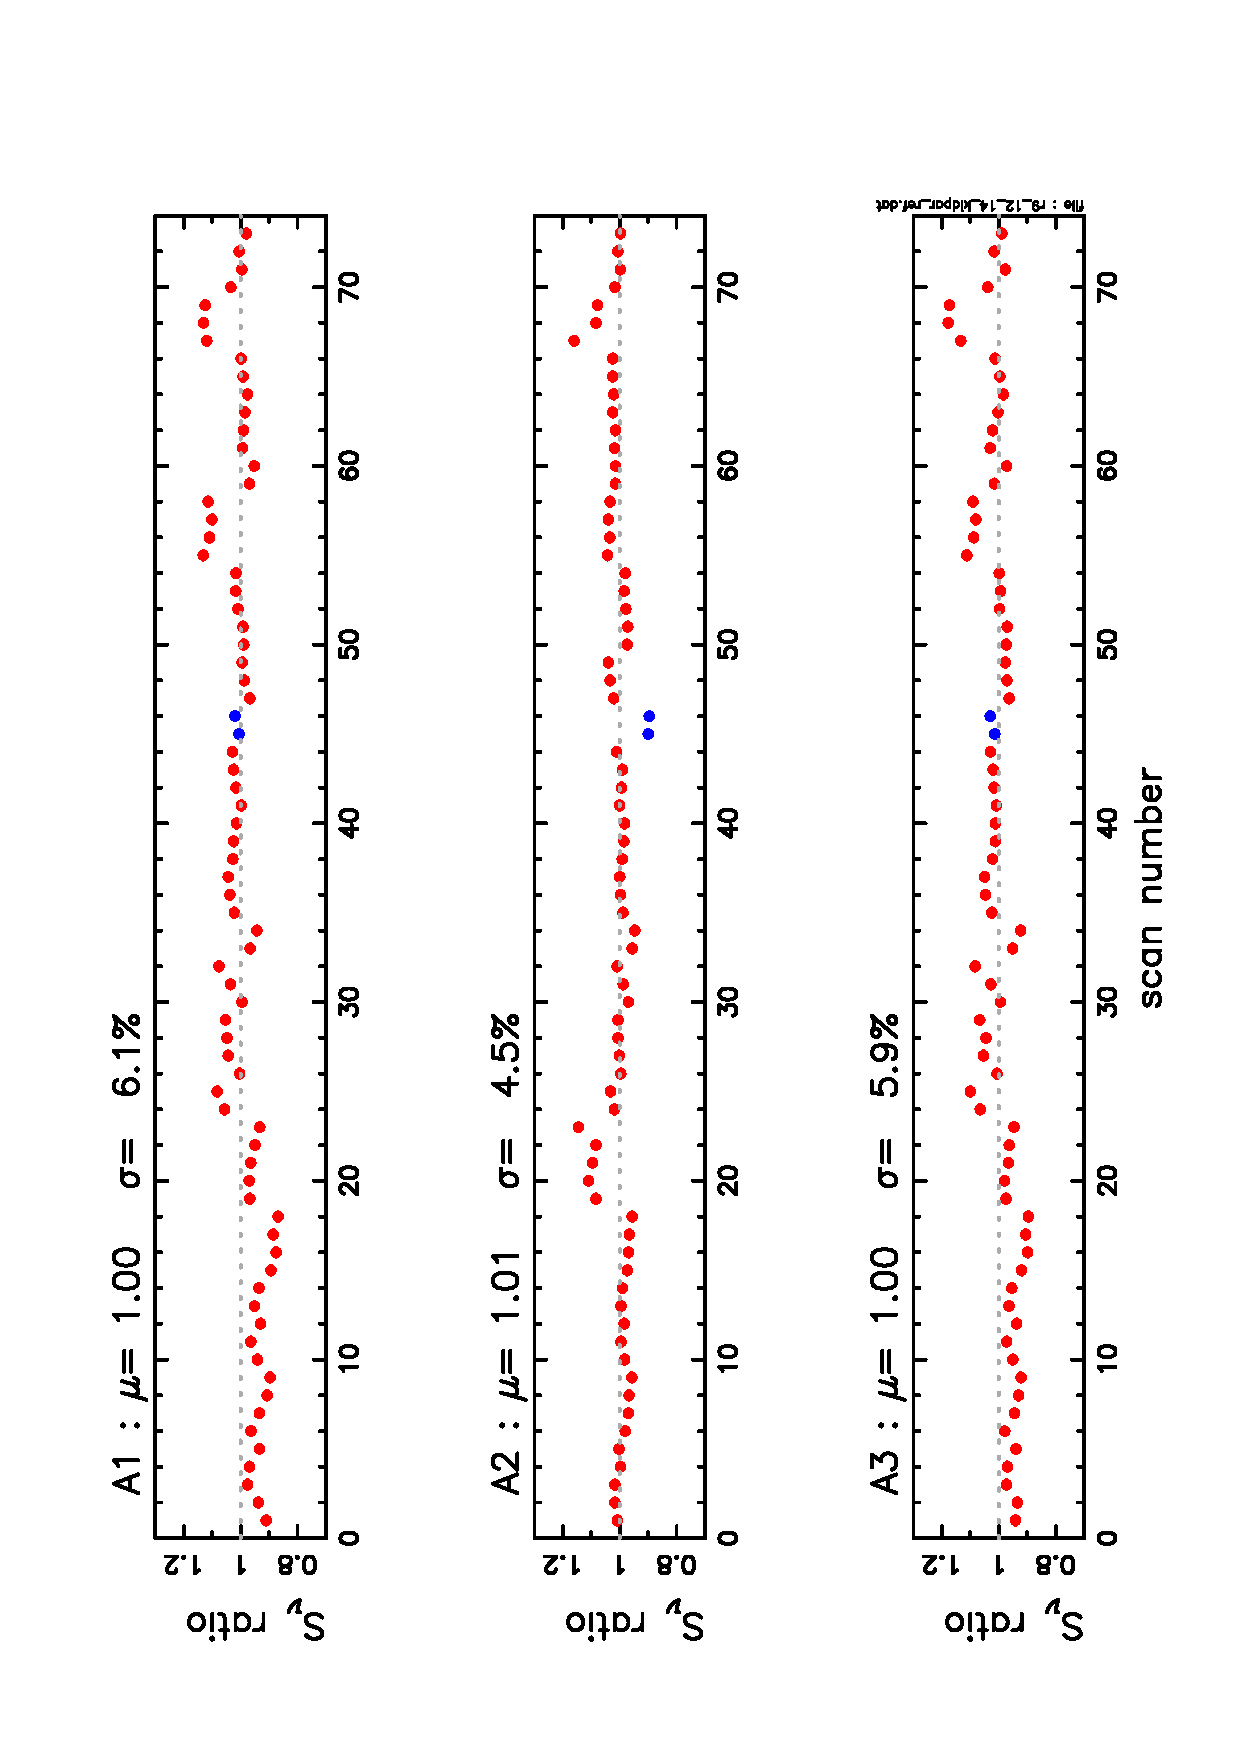
\includegraphics[clip=true,angle=-90.,width=0.85\textwidth]{Figures/Aperture_photo/Flux_ratio_index_A1_A2_A3_r9_r12_r14.pdf}
% \caption{Aperture photometry of Uranus (red) and Neptune (blue) observations during runs 9, 12 and 14 (displayed sequentially). Flux ratios ($\mu$) with respect to
% rference flux densities from planet atmospheric models at 260 and 150 GHz adopted to establish the  reference kidpars,  and scatters ($\sigma$), are given.}
% \label{fig:Uranus_s308}
%  \end{center}
%\end{figure}

\begin{table*}[!h]
\caption{ratio aperture photometry / fixed-width Gaussian flux densities   }
\label{tab:ratio}
\centering
\begin{tabular}{l| c | c c c }
\hline\hline
\noalign{\smallskip}
run     & Nber of scans  &  A1    &    A2   &  A3    \\
\hline
r9    & 27  &  1.08$\pm$ 0.03    &  1.04$\pm$ 0.02 & 1.09 $\pm$ 0.03     \\
r12   & 20  &  1.12$\pm$ 0.02    &  1.05$\pm$ 0.02 & 1.13 $\pm$ 0.02     \\
r14   & 28  &  1.09$\pm$ 0.03    &  1.03$\pm$ 0.02 & 1.09 $\pm$ 0.03     \\
\noalign{\smallskip}
\hline
\end{tabular}
\end{table*}
